\section{Remote modules}

\begin{frame}{About remote modules}
\begin{block}{What they are}
  \begin{itemize}
    \item Pieces of OTB code (filters, applications ...)
    \item That can be hosted one someone else git repository
    \item With a different licence
    \item While still being tested and packaged with OTB
    \item \url{gitlab.orfeo-toolbox.org/remote_modules/remote-module-template}
  \end{itemize}
\end{block}

\begin{block}{How people use them}
  \begin{itemize}
    \item A standard way to package new feature to share with other
    \item Ranging from small modules (1 filter, 1 app)
    \item ... to full processing chains as remote module
    \end{itemize}
\end{block}

  
\end{frame}

\begin{frame}{OTBTF: How deep is the OTB?}
  \begin{itemize}
  \item Remote  module developed by Remi Cresson (IRSTEA)
  \item Based on TensorFlow
  \item Provides all the plumbing perform Deep Learning based classification on Remote Sensing images:
    \begin{itemize}
      \item Generate training data from the OTB training data sampling framework
      \item Train your network (can also be done directly with TensorFlow)
      \item Serve the model (classify) on full remote sensing images with streaming
    \end{itemize}
    \item \url{gitlab.irstea.fr/remi.cresson/otbtf}
  \end{itemize}
\begin{center}
  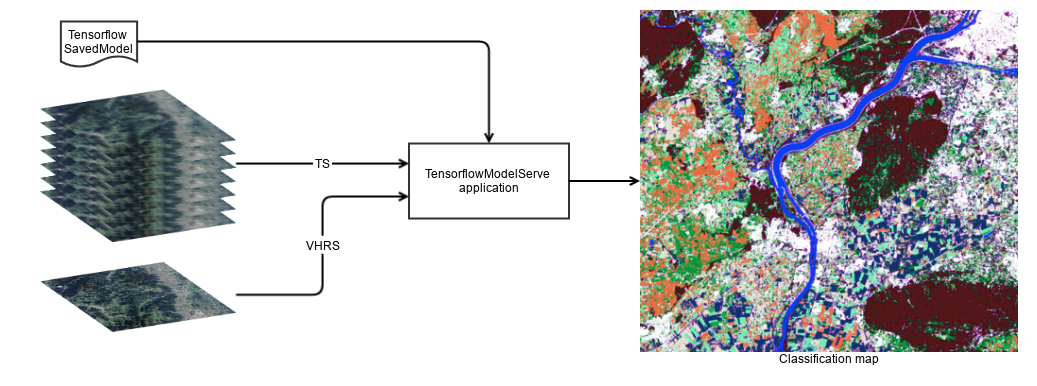
\includegraphics[width=0.8\textwidth]{images/classif_map.png}
\end{center}
\end{frame}
  
\begin{frame}{LSOBIA: Segment!}
  \begin{itemize}
    \item Remote module funded by CNES with contributions from Remi Cresson (IRSTEA)
    \item Baatz \& Shape segmentation \ldots
      \begin{itemize}
      \item Tilewise with an exact solution (no monkey stitching!)
      \item MPI-based cluster processing on several nodes
      \end{itemize}
    \item \url{https://github.com/RTOBIA/LSOBIA}
  \end{itemize}

  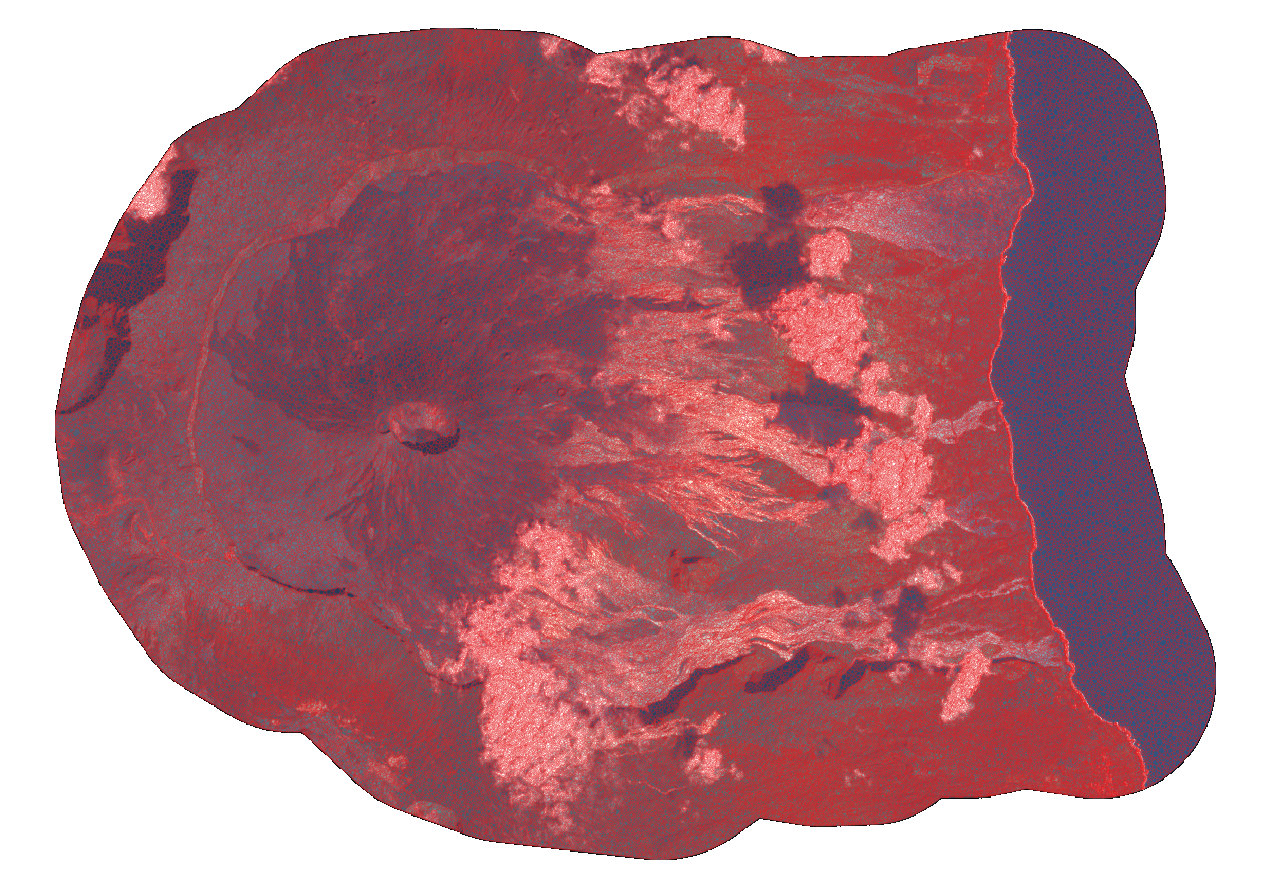
\includegraphics[width=0.5\textwidth]{images/seg_reunion.png}
  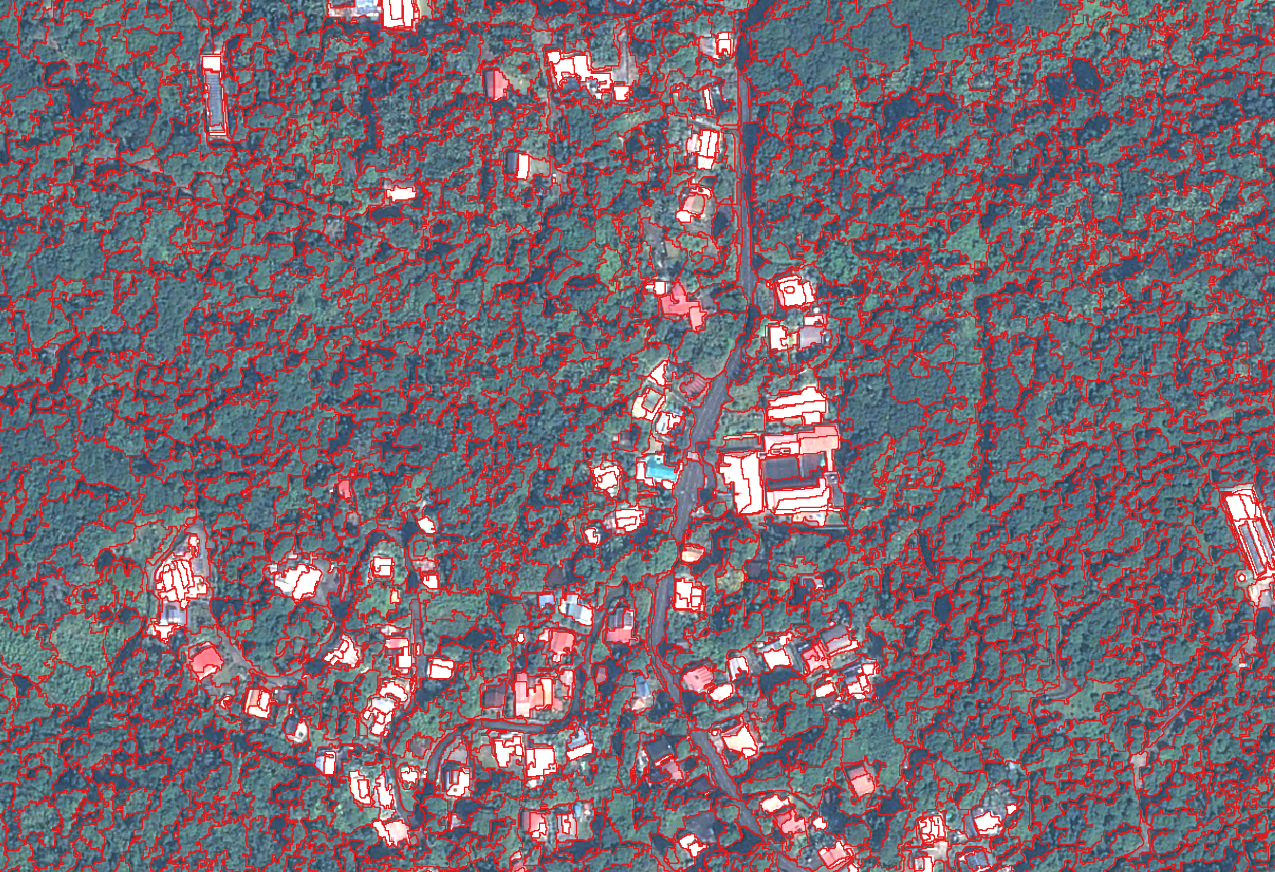
\includegraphics[width=0.5\textwidth]{images/seg_reunion_zoom.png}\\
  35129x25161 pixels: 3 221 860 polygons segmented in 16 minutes on 32 cluster nodes!


  
\end{frame}
  
\begin{frame}{Let It Snow: Snow mapping made easy}

  \begin{columns}
    \column{0.7\textwidth}
  \begin{itemize}
    \item 20m resolution snow cover maps from Sentinel2 (every 5 days)
    \item Code from CNES/CESBIO/CNRS
    \item Used for automatic production of selected sites on \url{theia.cnes.fr}: more than 900 products available!
  \end{itemize}
  \begin{center}
    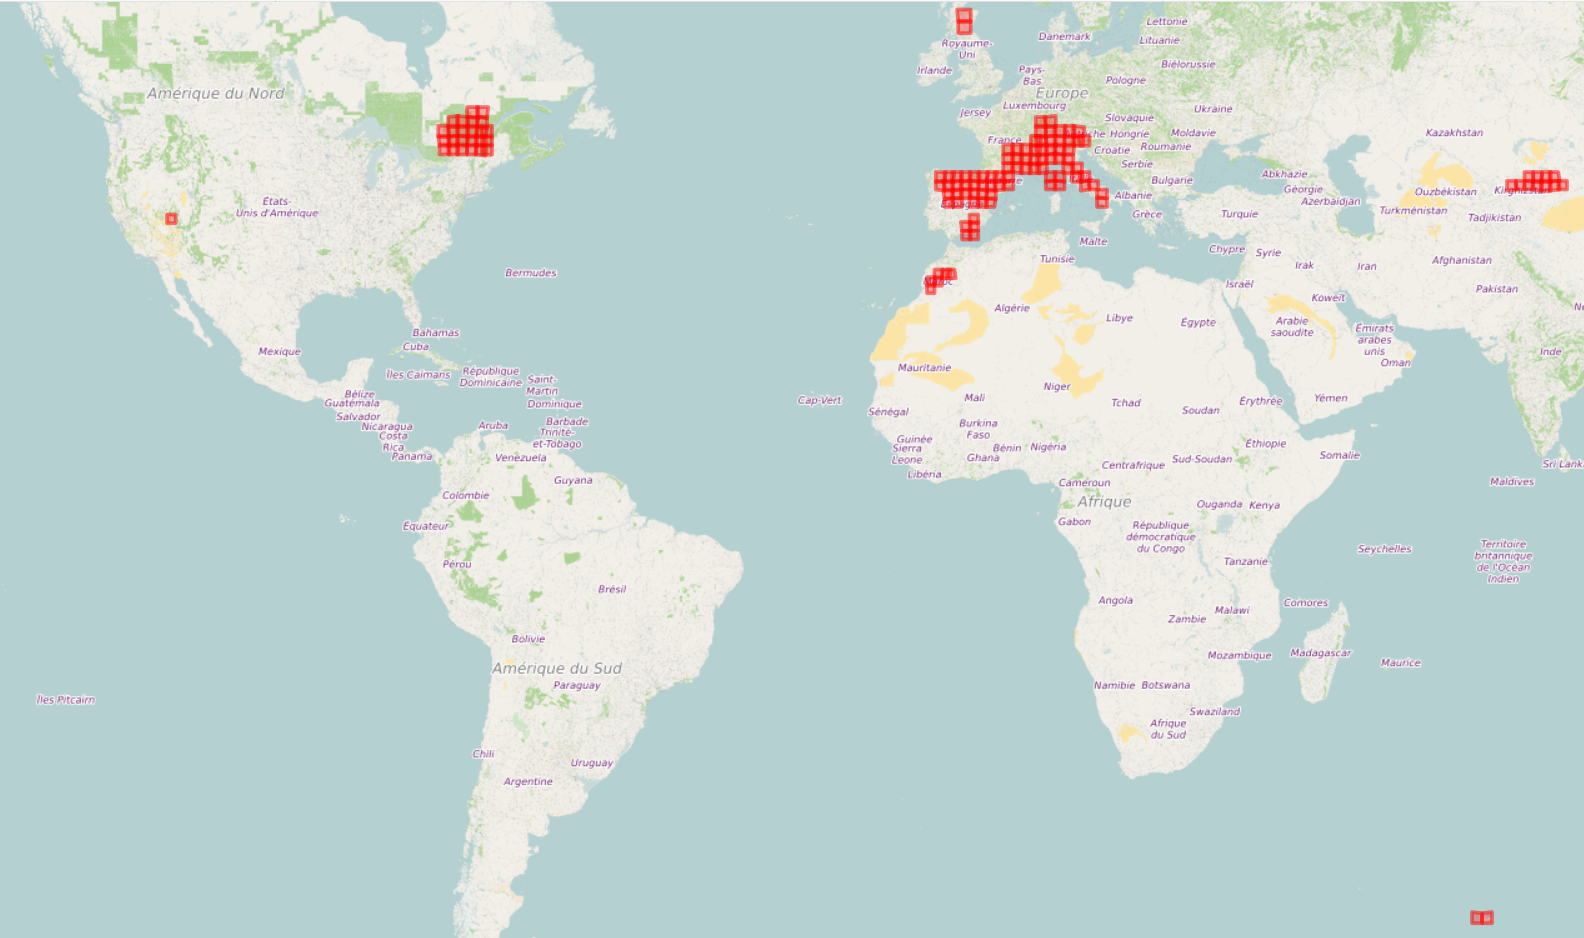
\includegraphics[width=0.7\textwidth]{images/lis-map.png}\\
    \begin{tiny}
      \url{tully.ups-tlse.fr/grizonnet/let-it-snow/tree/develop}\\
      \url{www.cesbio.ups-tlse.fr/multitemp/?cat=159}
    \end{tiny}
  \end{center}
  \column{0.3\textwidth}
  \begin{center}
    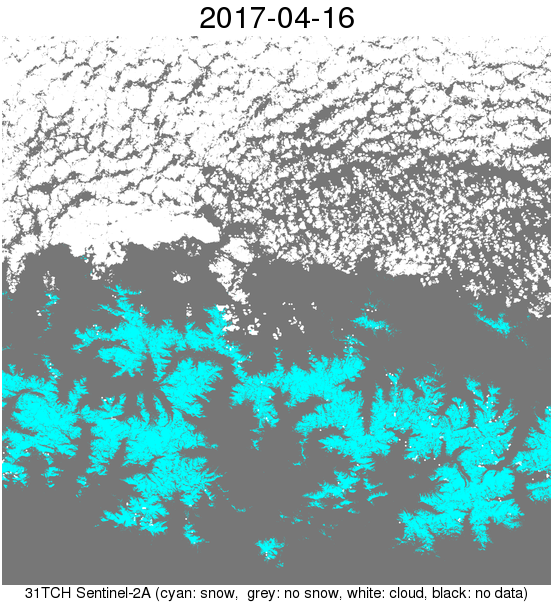
\includegraphics[width=0.95\textwidth]{images/lis-example.png}\\
    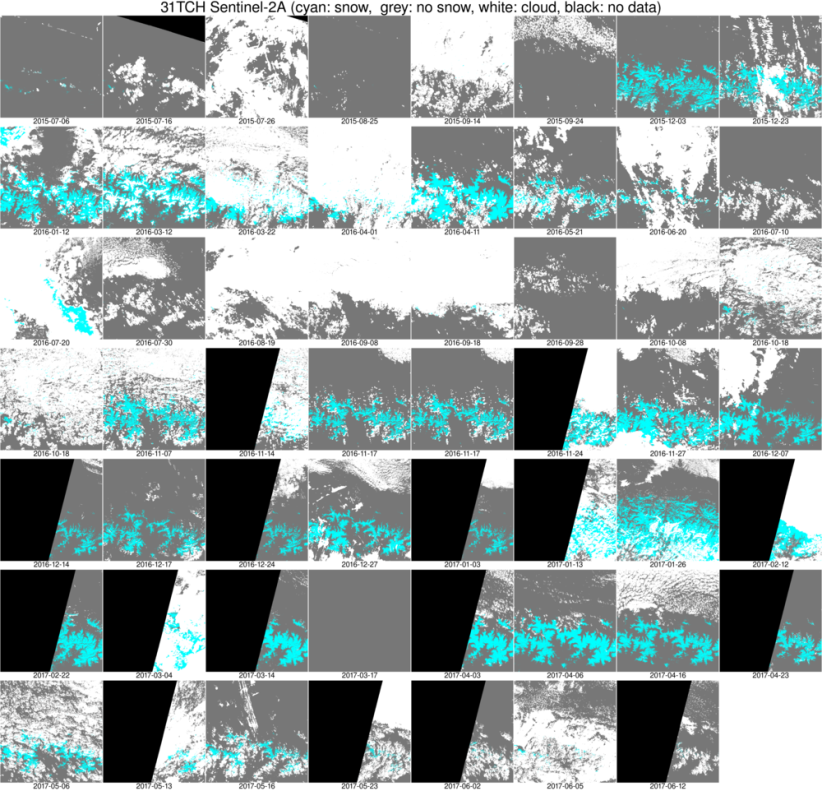
\includegraphics[width=0.95\textwidth]{images/lis-series.png}
    \end{center}
  \end{columns}


\end{frame}

\begin{frame}{Iota2: from images to country-scale land cover maps}
  \begin{itemize}
    \item Python/OTB  processing chain developed by CESBIO in the frame of Theia
    \item Able to produce country-scale land cover maps from Sentinel2/LandSat8 data
    \item Based on OTB reference data sampling and machine learning frameworks
    \item Runs on CNES HPC infrastructure
    \item \url{framagit.org/inglada/iota2}
    \item 2016: \url{osr-cesbio.ups-tlse.fr/~oso/posts/2017-03-30-carte-s2-2016/}
    \item 2017: \url{osr-cesbio.ups-tlse.fr/~oso/posts/2018-04-09-carte-s2-2017/}
      \begin{center}
        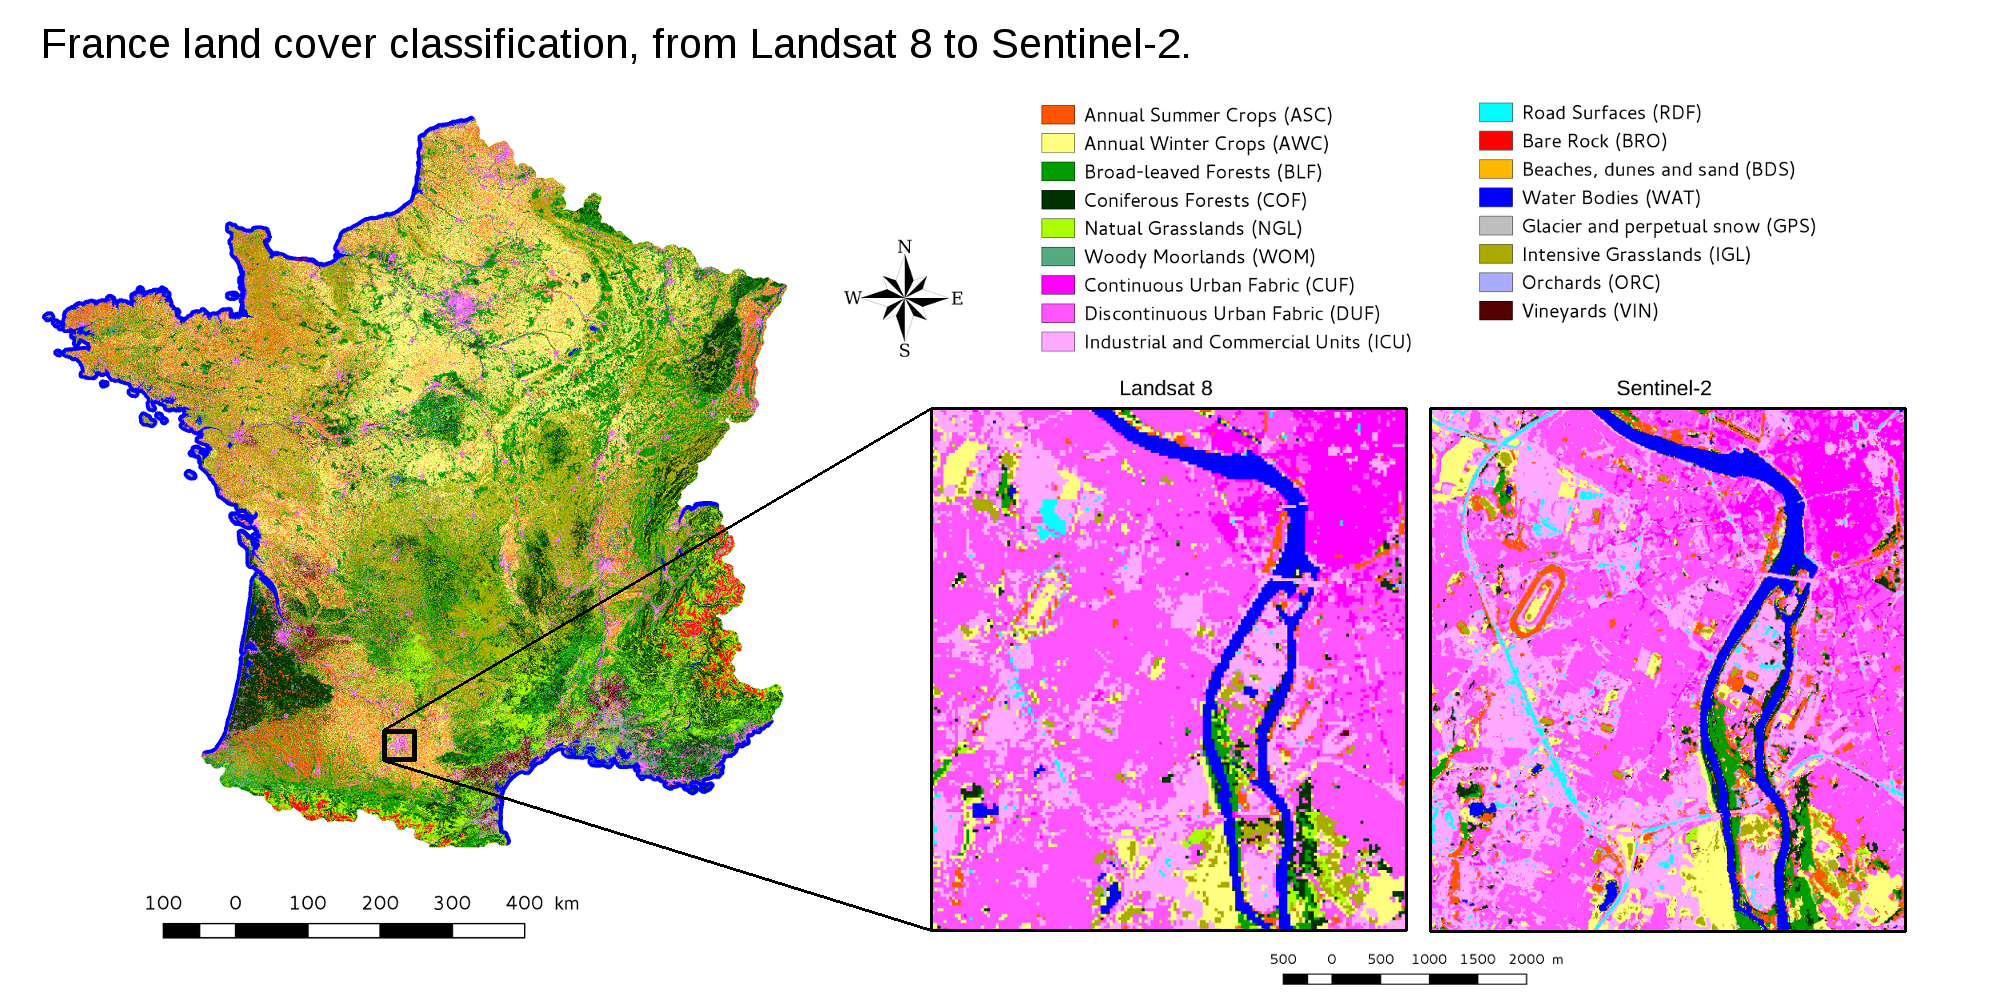
\includegraphics[width=0.7\textwidth]{images/oso-2016.png}
        \end{center}
  \end{itemize}
      
\end{frame}

\begin{frame}{DiapOTB: SAR interferometry in OTB}

  \begin{columns}
    \column{0.5\textwidth}
  \begin{itemize}
    \item WiP to port a legacy processing chain for SAR interferometry called Diapason
    \item As an Orfeo ToolBox remote module
    \item Funded by CNES  
    \item Coherence and interferogram time series from Sentinel1
    \item Phase unwrapping
    \item Support for S1 IW and other sensors
    \item \url{gitlab.orfeo-toolbox.org/remote_modules/diapotb}
  \end{itemize}
  \column{0.5\textwidth}
  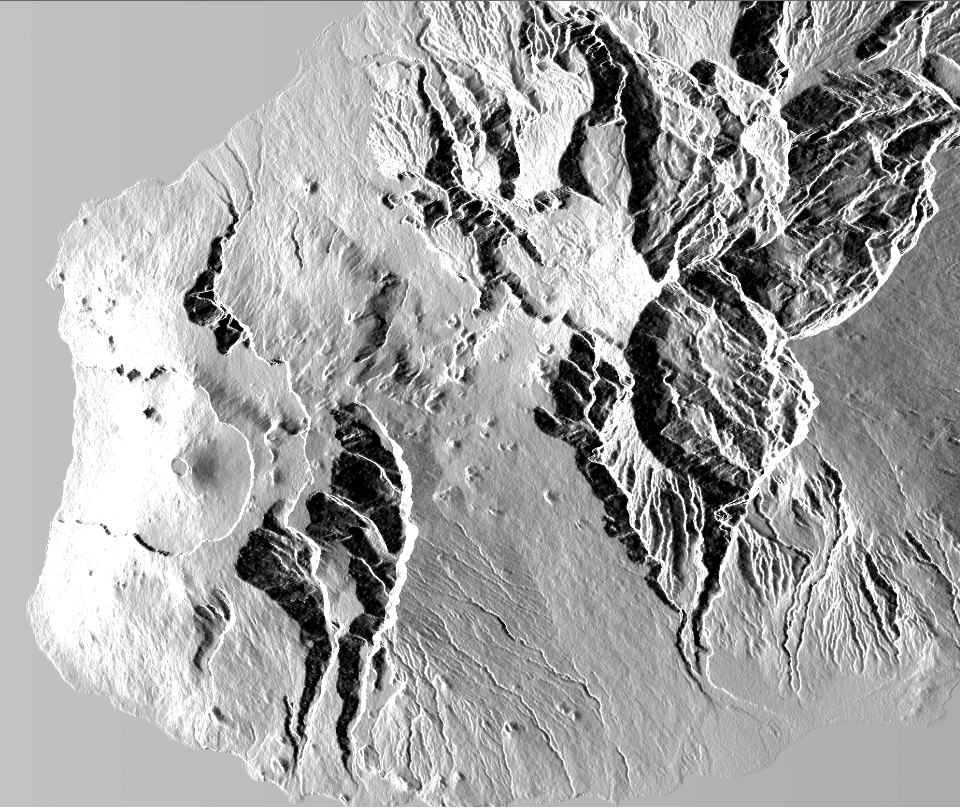
\includegraphics[width=\textwidth]{images/diapotb.png}\\
  \begin{tiny}
    Simulation of SAR image from Digital Elevation Model (part of the Diapason method)
    \end{tiny}
  \end{columns}
  
\end{frame}
